\documentclass[aspectratio=169, 10pt]{beamer}
\usetheme{Madrid}
\usecolortheme{seahorse}
\useinnertheme{rounded}

\usepackage{amsmath, amssymb}
\usepackage{tikz}
\usetikzlibrary{arrows.meta, positioning, shapes.geometric, fit, backgrounds}
\usepackage{booktabs}
\usepackage{xcolor}
\usepackage{graphicx}
% \usepackage{fontawesome5}  % removed --- not always available on Overleaf
\usepackage{tcolorbox}
\tcbuselibrary{skins, breakable}

% ── Colours ──────────────────────────────────────────────────────
\definecolor{physblue}{RGB}{31,  97, 141}
\definecolor{mlgreen} {RGB}{39, 174,  96}
\definecolor{warnred} {RGB}{192,  57,  43}
\definecolor{notegray}{RGB}{149, 165, 166}
\definecolor{lightyellow}{RGB}{255, 249, 219}

\setbeamercolor{block title}{bg=physblue, fg=white}
\setbeamercolor{block body} {bg=physblue!10}
\setbeamercolor{alertblock title}{bg=warnred, fg=white}
\setbeamercolor{alertblock body} {bg=warnred!10}
\setbeamercolor{exampleblock title}{bg=mlgreen!80!black, fg=white}
\setbeamercolor{exampleblock body} {bg=mlgreen!10}

% ── Helpers ──────────────────────────────────────────────────────
\newcommand{\tick}{\textcolor{mlgreen}{\checkmark}}
\newcommand{\cross}{\textcolor{warnred}{$\times$}}
\newcommand{\warn}{\textcolor{warnred}{$\triangle$!}}
\newcommand{\mytodo}{\textcolor{physblue}{$\diamond$}}

\newcommand{\highlight}[1]{\textcolor{physblue}{\textbf{#1}}}
\newcommand{\red}[1]{\textcolor{warnred}{\textbf{#1}}}

\title[Physics Evaluation for Interaction Motions]{%
  \textbf{Physics-Based Evaluation of\\Two-Person Interaction Motions}}
\subtitle{Supervisor Meeting}
\author{R H}
\date{March 25, 2026}
\institute{InterMask / Newton Physics Project}

% ─────────────────────────────────────────────────────────────────
\begin{document}
% ─────────────────────────────────────────────────────────────────

\begin{frame}
  \titlepage
\end{frame}

% ──────────────────────────────────────────────────────────────────
\section{Motivation}
% ──────────────────────────────────────────────────────────────────

\begin{frame}{Why Do Existing Metrics Fall Short?}
  \begin{columns}[T]
    \column{0.5\textwidth}
      \textbf{What InterMask already measures:}
      \vspace{0.3em}
      \begin{itemize}
        \item \tick\ \textbf{FID} --- distribution realism (feature space)
        \item \tick\ \textbf{MPJPE} --- joint position accuracy
        \item \tick\ \textbf{Diversity} --- variety of outputs
        \item \tick\ \textbf{R-precision} --- text--motion alignment
      \end{itemize}

      \vspace{0.8em}
      \begin{alertblock}{The gap}
        All of these are \emph{geometric}.\\
        They compare \textbf{where} body parts are\\
        but \emph{not} \textbf{how} the motion was produced.
      \end{alertblock}

    \column{0.5\textwidth}
      \textbf{What geometry cannot catch:}
      \vspace{0.3em}
      \begin{itemize}
        \item[\cross] Foot sliding (plausible pose, impossible contact)
        \item[\cross] Anti-gravity jumps (right position, wrong timing)
        \item[\cross] Interaction forces that violate Newton's laws\\
                      (e.g.\ one person ``pulls'' the other with no contact)
        \item[\cross] Impossible joint velocities / accelerations
      \end{itemize}

      \vspace{0.5em}
      % ── INSERT: side-by-side frame from a generated clip
      %    showing feet floating vs touching ground
      \begin{tcolorbox}[colback=lightyellow, colframe=notegray,
                        title={\small [IMG]Suggested figure}]
        \small Two frames from a generated clip:\\
        Left: geometrically plausible (low MPJPE)\\
        Right: feet floating 5 cm above ground
      \end{tcolorbox}
  \end{columns}
\end{frame}

% ──────────────────────────────────────────────────────────────────

\begin{frame}{Our Claim}
  \begin{center}
    \Large
    A motion that \emph{looks} realistic to a learned feature extractor\\[0.4em]
    may still be \highlight{physically impossible}.\\[1em]
    \normalsize
    We want to detect and quantify this gap.
  \end{center}

  \vspace{1em}
  \begin{block}{Proposed addition to the evaluation suite}
    \textbf{Dynamic Gap} $\Delta F_\text{sky}$: how much external ``magic'' force\\
    must be injected to maintain a generated trajectory vs.\ a GT trajectory.
  \end{block}

  \vspace{0.5em}
  \begin{center}
    $\underbrace{\Delta F_\text{sky} \approx 0}_{\text{GT mocap}}$
    \hspace{3em}
    $\underbrace{\Delta F_\text{sky} \gg 0}_{\text{physically impossible generation}}$
  \end{center}
\end{frame}

% ──────────────────────────────────────────────────────────────────
\section{Physics Background (Brief)}
% ──────────────────────────────────────────────────────────────────

\begin{frame}{What is a Torque?}
  \begin{columns}[T]
    \column{0.55\textwidth}
      \textbf{Torque $\tau$} = rotational force that drives a joint.\\[0.5em]

      Think of it as the ``effort'' a muscle group must produce to rotate
      a limb against gravity and inertia:
      \vspace{0.4em}
      \begin{itemize}
        \item \textbf{Knee joint}: quad/hamstring torque to stand from a squat
        \item \textbf{Shoulder joint}: deltoid torque to raise an arm
        \item \textbf{Hip joint}: glute torque during a kick
      \end{itemize}

      \vspace{0.6em}
      \begin{block}{Units}
        $\tau$ in \textbf{Newton-metres (Nm)}.\\
        Human joint limits: $\sim$10--150 Nm (hip $>$ wrist).
      \end{block}

      \vspace{0.4em}
      \textbf{Why it matters:}
      A motion is only physically possible if all joint torques
      stay within human capability and are \emph{consistent with contacts}.

    \column{0.45\textwidth}
      % ── INSERT: a stick figure with a torque arrow at the knee
      \begin{tcolorbox}[colback=lightyellow, colframe=notegray,
                        title={\small [IMG]Suggested figure}]
        \small Stick figure in squat:\\
        Arrow at knee showing torque direction.\\
        Label: ``$\tau_\text{knee} \approx 80\,\text{Nm}$''\\[0.5em]
        Same figure with feet 5 cm off ground:\\
        Label: ``$\tau_\text{root} \approx 800\,\text{N}$ (impossible)''
      \end{tcolorbox}

      \vspace{0.5em}
      \begin{tcolorbox}[colback=physblue!10, colframe=physblue]
        \small \textbf{Analogy:} Torque is to rotation as force is to translation.\\
        In deep learning terms: it is the ``gradient'' that the body applies
        to change joint angles.
      \end{tcolorbox}
  \end{columns}
\end{frame}

% ──────────────────────────────────────────────────────────────────

\begin{frame}{The Skyhook Problem --- Root Residuals}
  \begin{columns}[T]
    \column{0.55\textwidth}
      A rigid-body character has \textbf{6 root DOFs} (position + orientation).\\[0.5em]

      In \emph{inverse dynamics}: given observed motion $q(t)$, we solve for torques $\tau(t)$
      such that $M(q)\ddot{q} + C(q,\dot{q}) = \tau + J^\top f_c$.\\[0.5em]

      The \textbf{root DOFs are unactuated} (no muscle drives the pelvis directly) ---
      only gravity and contact forces act on it.\\[0.5em]

      \begin{alertblock}{Root residual = skyhook force}
        If the computed $\tau_\text{root} \neq 0$, it means we must inject
        a \textbf{virtual external force} to keep the character on its trajectory.\\
        Like suspending it from an invisible string --- a ``skyhook''.
      \end{alertblock}

    \column{0.45\textwidth}
      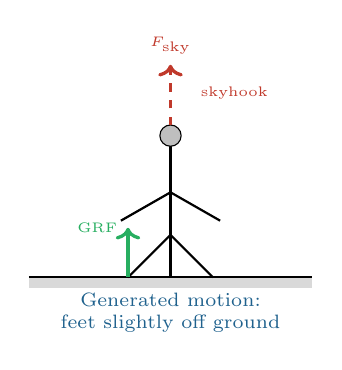
\begin{tikzpicture}[scale=0.9]
        % Ground
        \fill[gray!30] (0,0) rectangle (4, -0.15);
        \draw[thick] (0,0) -- (4,0);

        % Stick figure
        \draw[thick] (2, 0) -- (2, 0.6);     % legs
        \draw[thick] (2, 0.6) -- (2, 1.4);   % torso
        \draw[thick] (2, 1.4) -- (2, 1.85);  % neck
        \draw[fill=gray!50] (2, 2.0) circle (0.15); % head
        \draw[thick] (2, 1.2) -- (1.3, 0.8); % left arm
        \draw[thick] (2, 1.2) -- (2.7, 0.8); % right arm
        \draw[thick] (2, 0.6) -- (1.4, 0.0); % left leg
        \draw[thick] (2, 0.6) -- (2.6, 0.0); % right leg

        % Ground reaction force (GT case)
        \draw[->, very thick, mlgreen] (1.4, 0) -- (1.4, 0.7)
          node[left, font=\tiny] {GRF};

        % Skyhook (generated case)
        \draw[->, very thick, warnred, dashed] (2, 2.15) -- (2, 3.0)
          node[above, font=\tiny, warnred] {$F_\text{sky}$};
        \node[font=\tiny, warnred] at (2.9, 2.6) {skyhook};

        % Label
        \node[font=\scriptsize, physblue, align=center] at (2,-0.5)
          {Generated motion:\\feet slightly off ground};
      \end{tikzpicture}

      \vspace{0.4em}
      \small
      \textbf{GT mocap:} $F_\text{sky} \approx 50$--$150\,\text{N}$ (noise only)\\
      \textbf{Generated:} $F_\text{sky}$ can exceed $1000\,\text{N}$
  \end{columns}
\end{frame}

% ──────────────────────────────────────────────────────────────────
\section{Pipeline}
% ──────────────────────────────────────────────────────────────────

\begin{frame}{Full Evaluation Pipeline}
  \begin{center}
  \begin{tikzpicture}[
    node distance=0.35cm and 0.45cm,
    box/.style={draw, rounded corners, fill=physblue!15,
                minimum width=1.9cm, minimum height=0.65cm,
                font=\scriptsize, align=center},
    gen/.style={box, fill=mlgreen!15},
    out/.style={box, fill=warnred!20},
    arrow/.style={-Stealth, thick}
  ]
    % GT branch (top)
    \node[box] (gt)        {InterHuman\\GT mocap};
    \node[box, right=of gt] (gt_jq) {joint angles\\+ betas};
    \draw[arrow] (gt) -- (gt_jq);

    % Gen branch (bottom)
    \node[gen, below=0.6cm of gt]   (im)     {InterMask\\(text $\to$ motion)};
    \node[gen, right=of im]         (im_jq)  {joint angles\\+ betas};
    \draw[arrow] (im) -- (im_jq);

    % Shared retarget
    \node[box, right=0.9cm of gt_jq] (retarget)
      {\textbf{Retarget}\\to Newton\\rigid body};
    \draw[arrow] (gt_jq)  -- (retarget);
    \draw[arrow] (im_jq) -| (retarget);

    % ID
    \node[box, right=0.5cm of retarget] (id)
      {Inverse\\Dynamics\\$\tau(t)$};
    \draw[arrow] (retarget) -- (id);

    % Root residual
    \node[box, right=0.5cm of id] (sky)
      {Root\\Residual\\$F_\text{sky}$};
    \draw[arrow] (id) -- (sky);

    % Metric
    \node[out, right=0.5cm of sky] (metric)
      {\textbf{Dynamic Gap}\\$\Delta F_\text{sky}$};
    \draw[arrow] (sky) -- (metric);

    % Labels
    \node[font=\tiny, text=notegray, below=0.05cm of im]
      {conditioned on text prompt};
    \node[font=\tiny, text=notegray, above=0.05cm of gt]
      {InterHuman dataset};
    \node[font=\tiny, text=notegray, below=0.05cm of retarget]
      {0.00 cm MPJPE verified};
  \end{tikzpicture}
  \end{center}

  \vspace{0.2em}
  \begin{columns}[T]
    \column{0.5\textwidth}
      \begin{block}{Retargeting (prepare2)}
        \small SMPL-X betas $\to$ subject-specific skeleton\\
        Joint rotations transferred directly\\
        \textbf{Verified:} 0.00 cm MPJPE on all clips
      \end{block}
    \column{0.5\textwidth}
      \begin{block}{Inverse Dynamics (prepare2)}
        \small Given $q(t)$, compute $\tau(t)$ analytically.\\
        B-spline smoothing (no noise amplification).\\
        \textbf{Fast:} $<1$\,s per 100-frame clip.
      \end{block}
  \end{columns}
\end{frame}

% ──────────────────────────────────────────────────────────────────

\begin{frame}{Metric Definition: Dynamic Gap}
  \begin{block}{Per-clip residual wrench}
    \vspace{0.3em}
    \[
      F_\text{sky}^{(c)} = \frac{1}{T}\sum_{t=1}^{T} \|\tau_\text{root}(t)\|_2
      \quad \text{[Newtons, per clip } c \text{]}
    \]
  \end{block}

  \vspace{0.4em}
  \begin{block}{Dynamic Gap (primary metric)}
    \vspace{0.3em}
    \[
      \Delta F_\text{sky} = \underbrace{F_\text{sky}^\text{gen}}_{\text{generated}} -
                            \underbrace{F_\text{sky}^\text{gt}}_{\text{GT}}
      \qquad \text{(per matching clip pair)}
    \]
    \vspace{-0.3em}
    \[
      \text{Dynamic Gap} = \mathbb{E}_c[\Delta F_\text{sky}(c)]
    \]
  \end{block}

  \vspace{0.4em}
  \begin{columns}[T]
    \column{0.33\textwidth}
      \begin{exampleblock}{GT reference}
        $F_\text{sky}^\text{gt} \approx 50\text{--}150\,\text{N}$\\
        (mocap noise + foot model)
      \end{exampleblock}
    \column{0.33\textwidth}
      \begin{alertblock}{Generated}
        $F_\text{sky}^\text{gen}$ can exceed $1000\,\text{N}$\\
        for physically impossible motions
      \end{alertblock}
    \column{0.33\textwidth}
      \begin{block}{Threshold}
        $F_\text{sky} > 3 \times mg \approx 2200\,\text{N}$\\
        = \textbf{impossible} frame\\
        (no athletic GRF can match this)
      \end{block}
  \end{columns}

  \vspace{0.3em}
  \small \textbf{Why relative?} Retargeting + ID introduce systematic bias on \emph{all} clips.
  $\Delta F_\text{sky}$ cancels it and isolates the generation artefact.
\end{frame}

% ──────────────────────────────────────────────────────────────────
\section{Differentiable Physics Tracker}
% ──────────────────────────────────────────────────────────────────

\begin{frame}{Beyond Inverse Dynamics: Physics Tracking}
  \begin{columns}[T]
    \column{0.56\textwidth}
      \small
      Inverse dynamics is \emph{open-loop}: it ignores contact consistency.\\
      Stronger test: can a controller \textbf{track} the motion in simulation?\\[0.4em]

      \textbf{Approach (PHC-inspired):} learn per-frame residuals $\Delta q$:
      \[
        \mathcal{L} = \|\text{sim\_pos}(t) - \text{ref\_pos}(t)\|^2 + \lambda \|\Delta q\|^2
      \]
      Backprop \emph{through} Newton's differentiable physics solver.\\[0.4em]

      \textbf{Analogous to:}
      \begin{itemize}\setlength\itemsep{0pt}
        \item Neural ODE backprop (ODE = rigid-body physics)
        \item Differentiable rendering (for articulated bodies)
      \end{itemize}

      \vspace{0.3em}
      \begin{exampleblock}{\small Tracking error as metric}
        \small GT: easier to track $\Rightarrow$ lower error\\
        Generated: harder $\Rightarrow$ higher error\\
        \textbf{Gap} = physics plausibility signal
      \end{exampleblock}

    \column{0.44\textwidth}
      \vspace{0.3em}
      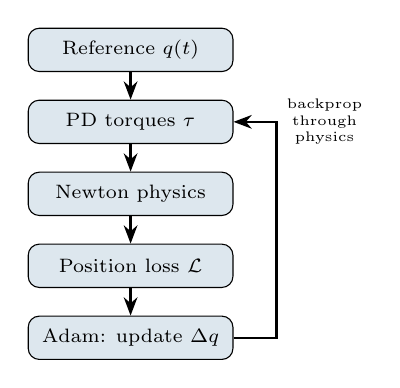
\begin{tikzpicture}[scale=0.78,
        box/.style={draw, rounded corners, fill=physblue!15, minimum width=2.6cm,
                    minimum height=0.55cm, font=\scriptsize, align=center},
        arrow/.style={-Stealth, thick}
      ]
        \node[box] (ref)  {Reference $q(t)$};
        \node[box, below=0.35cm of ref]  (pd)   {PD torques $\tau$};
        \node[box, below=0.35cm of pd]   (sim)  {Newton physics};
        \node[box, below=0.35cm of sim]  (loss) {Position loss $\mathcal{L}$};
        \node[box, below=0.35cm of loss] (adam) {Adam: update $\Delta q$};

        \draw[arrow] (ref) -- (pd);
        \draw[arrow] (pd)  -- (sim);
        \draw[arrow] (sim) -- (loss);
        \draw[arrow] (loss)-- (adam);
        \draw[arrow] (adam.east) -- ++(0.7,0) |- (pd.east)
          node[midway, right, font=\tiny, align=center] {backprop\\through\\physics};
      \end{tikzpicture}
    \end{columns}
\end{frame}

% ──────────────────────────────────────────────────────────────────
\section{Results \& Problems}
% ──────────────────────────────────────────────────────────────────

\begin{frame}{Preliminary Results}
  \begin{columns}[T]
    \column{0.5\textwidth}
      \textbf{Retargeting accuracy:}
      \begin{itemize}
        \item[\tick] 0.00 cm MPJPE on all clips
        \item[\tick] Per-subject body proportions (SMPL-X betas)
        \item[\tick] Foot contact geometry calibrated
      \end{itemize}

      \vspace{0.6em}
      \textbf{PHC tracker (clip 1129, 20 epochs):}
      \begin{center}
      \begin{tabular}{lc}
        \toprule
        Source & MPJPE \\
        \midrule
        GT motion & $\sim$150 mm \\
        Generated  & $\sim$193 mm \\
        \bottomrule
      \end{tabular}
      \end{center}
      \small Gap is the signal; absolute values will decrease with more training.

    \column{0.5\textwidth}
      \textbf{Differentiable optimizer speed (clip 1129):}
      \begin{center}
      \begin{tabular}{lcc}
        \toprule
        Config & Time/window & 20 epochs \\
        \midrule
        16 substeps (old) & $\sim$4 min & $\sim$1400 min \\
        \textbf{4 substeps (new)} & \textbf{20 s} & \textbf{$\sim$138 min} \\
        \bottomrule
      \end{tabular}
      \end{center}
      \small 10$\times$ speedup. Gradients confirmed flowing (grad\_norm = 0.57).

      \vspace{0.5em}
      % ── INSERT: loss curve over 20 epochs
      \begin{tcolorbox}[colback=lightyellow, colframe=notegray,
                        title={\small [IMG]Suggested figure}]
        \small Loss curve: GT vs Generated tracking loss over 20 epochs
      \end{tcolorbox}
  \end{columns}
\end{frame}

% ──────────────────────────────────────────────────────────────────

\begin{frame}{Open Problems}
  \small
  \begin{enumerate}\setlength\itemsep{0.4em}
    \item \warn\ \textbf{Optimizer is still slow.}
    Backward $\approx 6\times$ forward; 138 min/clip $\times$ 200 clips = impractical.\\
    \textit{Options:} truncated BPTT, shrinking window, kinematic warm-start.

    \item \warn\ \textbf{Tracker not yet converging on GT.}
    GT MPJPE $\sim$150 mm after 20 epochs (target $<$50 mm).\\
    Likely: PD gains not tuned for SMPL-X, sphere foot approximation.

    \item \warn\ \textbf{GT motions have non-zero residual wrenches.}
    Even real mocap needs $\sim$100--300 N skyhook (noise + retargeting).\\
    \textbf{Fix:} use $\Delta F_\text{sky} = F^\text{gen} - F^\text{gt}$ --- systematic bias cancels.

    \item \warn\ \textbf{Dataset-scale evaluation is slow.}
    Full 200-clip eval takes hours even with 2$\times$ RTX 3090.\\
    \textbf{Current plan:} 50-clip stratified proxy + multi-GPU parallelism.
  \end{enumerate}
\end{frame}

% ──────────────────────────────────────────────────────────────────

\begin{frame}{Visual Explanation: What the Metric Detects}
  \begin{columns}[T]
    \column{0.5\textwidth}
      % ── INSERT: side by side Newton viewer screenshot GT vs gen
      \begin{tcolorbox}[colback=lightyellow, colframe=notegray,
                        title={\small [IMG]Figure A --- Newton viewer}]
        \small \textbf{Left:} GT motion replayed in Newton.\\
        Feet firmly on ground.\\
        Low skyhook force ($F_\text{sky} \approx 80\,\text{N}$).\\[0.4em]
        \textbf{Right:} Generated motion replayed.\\
        Feet floating / penetrating floor.\\
        High skyhook force ($F_\text{sky} \approx 600\,\text{N}$).\\[0.4em]
        \textit{Ask: can you record this from the Newton viewer?}
      \end{tcolorbox}

    \column{0.5\textwidth}
      % ── INSERT: torque / skyhook force time series plot
      \begin{tcolorbox}[colback=lightyellow, colframe=notegray,
                        title={\small [IMG]Figure B --- Force time series}]
        \small Time-series plot (already generated by pipeline):\\
        \texttt{output/newton\_pd\_forward/clip\_1129\_hit/}\\
        \texttt{root\_residuals.png}\\[0.4em]
        Shows: GT root PD forces vs generated.\\
        \textit{Copy this figure here.}
      \end{tcolorbox}

      \vspace{0.5em}
      % ── INSERT: histogram ΔF_sky
      \begin{tcolorbox}[colback=lightyellow, colframe=notegray,
                        title={\small [IMG]Figure C --- $\Delta F_\text{sky}$ histogram}]
        \small Histogram over 50 test clips:\\
        $\Delta F_\text{sky} = F_\text{sky}^\text{gen} - F_\text{sky}^\text{gt}$\\
        Expected: distribution shifted right (gen $>$ GT).
      \end{tcolorbox}
  \end{columns}
\end{frame}

% ──────────────────────────────────────────────────────────────────
\section{Discussion \& Next Steps}
% ──────────────────────────────────────────────────────────────────

\begin{frame}{Discussion Questions}
  \small
  \begin{enumerate}\setlength\itemsep{0.5em}
    \item \textbf{Is the residual wrench metric enough for a contribution,} or do we need full tracking?\\
          Wrench: fast, no optimisation, interpretable (physical units).\\
          Tracking: stronger claim, but slow and not yet converged.

    \item \textbf{Should we compare against existing physics-based work?}\\
          PhysDiff, PULSE, PHC --- all single-person only; no two-person equivalent exists.

    \item \textbf{Scope question:}
          \begin{itemize}\setlength\itemsep{0pt}
            \item Metric only (evaluation paper)?
            \item Metric + physics-guided post-processing?
            \item Compare InterMask vs.\ InterGen vs.\ ReInteract?
          \end{itemize}

    \item \textbf{Compute:} 2$\times$ RTX 3090, $\sim$6h for 200-clip eval.\\
          Is cluster access available for full ablation?
  \end{enumerate}
\end{frame}

% ──────────────────────────────────────────────────────────────────

\begin{frame}{Next Steps}
  \begin{center}
  \begin{tabular}{clcc}
    \toprule
    \textbf{Priority} & \textbf{Task} & \textbf{Status} & \textbf{Est.} \\
    \midrule
    \highlight{HIGH} & Run residual wrench eval on 50 test clips & Ready & 1 day \\
    \highlight{HIGH} & Tune PHC tracker gains $\to$ GT MPJPE $<$50 mm & In progress & 2--3 days \\
    \highlight{MED} & Truncated BPTT for faster optimization & Planned & 1 week \\
    \highlight{MED} & $\Delta F_\text{sky}$ comparison: GT vs InterMask & Ready & 2 days \\
    \highlight{LOW} & Full test-set evaluation (200 clips) & Blocked by speed & 2 weeks \\
    \bottomrule
  \end{tabular}
  \end{center}

  \vspace{0.8em}
  \begin{block}{Immediate deliverable}
    Within 1 week: a $\Delta F_\text{sky}$ comparison plot over 50 test clips,
    showing that generated motions have statistically higher residual root forces than GT.
  \end{block}
\end{frame}

% ──────────────────────────────────────────────────────────────────

\begin{frame}{Summary}
  \begin{columns}[T]
    \column{0.5\textwidth}
      \textbf{What we have:}
      \begin{itemize}
        \item[\tick] Perfect retargeting (0 cm MPJPE)
        \item[\tick] Fast inverse dynamics pipeline
        \item[\tick] Residual wrench metric (Dynamic Gap)
        \item[\tick] Differentiable physics tracker (prototype)
        \item[\tick] 10$\times$ optimizer speedup validated
      \end{itemize}

    \column{0.5\textwidth}
      \textbf{The key idea:}
      \begin{itemize}
        \item[$\rightarrow$] Generated motions look plausible geometrically
        \item[$\rightarrow$] But require unrealistic external forces to be physically realised
        \item[$\rightarrow$] $\Delta F_\text{sky}$ quantifies this gap
        \item[$\rightarrow$] Complements FID/MPJPE with a physics-grounded signal
      \end{itemize}
  \end{columns}

  \vspace{1em}
  \begin{center}
    \Large \highlight{Goal:} The first physics-based evaluation metric\\
    for \textbf{two-person interaction motion generation}.
  \end{center}
\end{frame}

% ──────────────────────────────────────────────────────────────────

\begin{frame}{Experiments Conducted --- Code Overview}
  \begin{columns}[T]
    \column{0.5\textwidth}
      \begin{block}{\texttt{prepare2} --- Analytical ID metric}
        \small
        Retarget SMPL-X to Newton skeleton.\\
        Inverse dynamics via B-spline differentiation.\\
        \textbf{Output:} root residual $F_\text{sky}$ per clip.\\
        \textbf{Status:} working, fast ($<$1s/clip).
      \end{block}

      \vspace{0.4em}
      \begin{block}{\texttt{prepare4} --- PD forward simulation}
        \small
        Replace ID with forward sim + PD tracking.\\
        Eliminates skyhook artefacts from ID.\\
        Torques from \texttt{pd\_torque\_kernel} at 480 Hz.\\
        \textbf{Status:} working; produces torque videos.
      \end{block}

    \column{0.5\textwidth}
      \begin{block}{\texttt{prepare5} --- Differentiable tracker (PHC-style)}
        \small
        Backprop through Newton SolverFeatherstone.\\
        Learns per-frame PD residuals $\Delta q$.\\
        10$\times$ speedup: 4 substeps (120 Hz) vs.\ 16.\\
        \textbf{Status:} prototype; MPJPE GT=150mm vs.\ Gen=193mm.
      \end{block}

      \vspace{0.4em}
      \begin{alertblock}{PPMotion metric (attempted)}
        \small
        Recreate PPMotion (Peng et al.) physics-based\\
        motion quality score for two-person setting.\\
        \textbf{Problem:} PPMotion assumes single person;\\
        interaction forces between persons not handled.\\
        \textbf{Status:} blocked --- defining our own metric instead.
      \end{alertblock}
  \end{columns}
\end{frame}

\begin{frame}[plain]
  \begin{center}
    \vspace{1.5cm}
    {\LARGE Thank you}\\[1em]
    \large Questions?\\[2em]
    \small
    \begin{tabular}{ll}
      Analytical metric: & \texttt{prepare2/} (ID + root residual) \\
      PD forward sim:    & \texttt{prepare4/} (480 Hz, torque videos) \\
      Diff.\ tracker:    & \texttt{prepare5/} (Newton backprop) \\
      Physics sim:       & Newton (NVIDIA Warp, differentiable) \\
      Body model:        & SMPL-X (55 joints, 10 shape betas) \\
    \end{tabular}
  \end{center}
\end{frame}

% ──────────────────────────────────────────────────────────────────
% APPENDIX
% ──────────────────────────────────────────────────────────────────

\appendix

\begin{frame}[allowframebreaks]{Appendix: Key Equations}
  \textbf{Equations of motion (rigid-body articulation):}
  \[
    M(q)\ddot{q} + C(q, \dot{q}) = \tau + J_c^\top f_c
  \]
  where $q \in \mathbb{R}^{76}$ (joint coords), $\tau \in \mathbb{R}^{75}$ (torques),
  $f_c$ (contact forces), $J_c$ (contact Jacobian).

  \vspace{0.8em}
  \textbf{Root residual (skyhook) from inverse dynamics:}
  \[
    \tau_\text{root}(t) = \left[M(q)\ddot{q} + C(q,\dot{q})\right]_{0:6}
    \quad \text{(with } f_c = 0 \text{ in naive ID)}
  \]
  For a motion that respects ground contact, $\|\tau_\text{root}\| \approx 0$.

  \vspace{0.8em}
  \textbf{PD torque (differentiable tracker):}
  \[
    \tau_j(t) = K_{p,j}\bigl(q_j^\text{ref}(t) + \Delta q_j(t) - q_j^\text{sim}(t)\bigr)
              - K_{d,j}\,\dot{q}_j^\text{sim}(t)
  \]
  $\Delta q_j$ is the learnable residual, optimised via backprop through Newton's
  SolverFeatherstone.

  \framebreak

  \textbf{Optimisation objective:}
  \[
    \min_{\Delta q} \sum_{t=1}^{T} \sum_{j=1}^{N_\text{joints}}
    \|p_j^\text{sim}(t) - p_j^\text{ref}(t)\|^2
    + \lambda \|\Delta q(t)\|^2
  \]

  \textbf{Window-based rollout:}
  Forward simulate $W$ frames, backprop tape, Adam step on $\Delta q$.
  Slide window across full clip ($\sim$21 windows for a 100-frame clip at $W=5$).
\end{frame}

\begin{frame}{Appendix: System Details}
  \begin{columns}[T]
    \column{0.5\textwidth}
      \textbf{Physics simulator:}
      \begin{itemize}
        \item Newton (NVIDIA, Warp-based)
        \item SolverFeatherstone (fully differentiable)
        \item 480 Hz physics, 30 fps control (16 substeps)
        \item Reduced to 120 Hz (4 substeps) for optimization
      \end{itemize}

      \vspace{0.5em}
      \textbf{Body model:}
      \begin{itemize}
        \item SMPL-X: 55 joints, 10 betas (shape params)
        \item Retargeted to 24-body rigid articulation
        \item Per-subject XML generated from betas
        \item Sphere feet for contact stability
      \end{itemize}

    \column{0.5\textwidth}
      \textbf{Hardware:}
      \begin{itemize}
        \item 2$\times$ NVIDIA RTX 3090 (24 GB each)
        \item Multi-GPU batch via Python multiprocessing
      \end{itemize}

      \vspace{0.5em}
      \textbf{Dataset:}
      \begin{itemize}
        \item InterHuman: $\sim$6800 clips (train/val/test)
        \item Test split: $\sim$500 clips
        \item Evaluation target: 200 clips (GT + generated)
      \end{itemize}
  \end{columns}
\end{frame}

\end{document}
